\documentclass{article}
\usepackage[a4paper, total={6in, 8in}]{geometry}
%\usepackage{multicol,lipsum}
\usepackage[toc,page]{appendix}
\setcounter{secnumdepth}{3} 
\usepackage[english]{babel}
\usepackage[utf8x]{inputenc}
\usepackage[T1]{fontenc}
\usepackage{float}
\usepackage{pdfpages}
\usepackage{xcolor}
\usepackage[hyperfootnotes=false]{hyperref}           % Enable embedded hyperlinks.

\usepackage{graphicx}	        % Enable for eps and pdf figures, if they occur
\DeclareGraphicsExtensions{.pdf,.png,.jpg}

\usepackage{grffile} %per risolvere il problema di immagini con molti . prima dell'estensione

\hypersetup{
    colorlinks=true,
    linkcolor=blue,
    filecolor=magenta,      
    urlcolor=cyan,
}
 
\urlstyle{same}

%\usepackage[bottom]{footmisc}
\usepackage[bottom, flushmargin]{footmisc}
\usepackage{footnotebackref}

\usepackage{rotating}
\usepackage{tikz}

\usepackage{listingsutf8}   		% Enable to use accent in Source code comment.
 \usepackage{listings}
 \usepackage{caption}
\usepackage{color}				% Eclipse style color
\definecolor{javared}{rgb}{0.6,0,0} % for strings
\definecolor{javagreen}{rgb}{0.25,0.5,0.35} % comments
\definecolor{javapurple}{rgb}{0.5,0,0.35} % keywords
\definecolor{javadocblue}{rgb}{0.25,0.35,0.75} % javadoc
 \definecolor{bkcolour}{rgb}{0.95,0.95,0.92}
\lstset{
%inputencoding=utf8/latin1,	% Enable to use accent in source code comment
%breaklines=true,				% Enable to avoid the source code exit the length of the page
%language=sh,
%backgroundcolor=\color{bkcolour},
%basicstyle=\ttfamily,
%keywordstyle=\color{javapurple}\bfseries,
%stringstyle=\color{javared},
%commentstyle=\color{javagreen},
%morecomment=[s][\color{javadocblue}]{#}{#},
%numbers=left,
%numberstyle=\tiny\color{black},
%stepnumber=2,
%numbersep=70pt,
%%%showstringspaces=false
}

%\usepackage[hmarginratio=1:1,top=32mm,columnsep=20pt]{geometry} % Document margins
%\usepackage[hang, small,labelfont=bf,up,textfont=it,up]{caption} % Custom captions under/above floats in tables or figures
%\usepackage{booktabs} % Horizontal rules in tables

\colorlet{punct}{red!60!black}
\definecolor{background}{HTML}{EEEEEE}
\definecolor{delim}{RGB}{20,105,176}
\colorlet{numb}{magenta!60!black}

\lstdefinelanguage{json}{
    basicstyle=\footnotesize\ttfamily,
    %numbers=left,
    numberstyle=\scriptsize,
    %stepnumber=1,
    numbersep=5pt,
    showstringspaces=false,
    %breaklines=true,
    %frame=lines,
    %backgroundcolor=\color{background},
    literate=
     *{0}{{{\color{numb}0}}}{1}
      {1}{{{\color{numb}1}}}{1}
      {2}{{{\color{numb}2}}}{1}
      {3}{{{\color{numb}3}}}{1}
      {4}{{{\color{numb}4}}}{1}
      {5}{{{\color{numb}5}}}{1}
      {6}{{{\color{numb}6}}}{1}
      {7}{{{\color{numb}7}}}{1}
      {8}{{{\color{numb}8}}}{1}
      {9}{{{\color{numb}9}}}{1}
      {:}{{{\color{punct}{:}}}}{1}
      {,}{{{\color{punct}{,}}}}{1}
      {\{}{{{\color{delim}{\{}}}}{1}
      {\}}{{{\color{delim}{\}}}}}{1}
      {[}{{{\color{delim}{[}}}}{1}
      {]}{{{\color{delim}{]}}}}{1},
}

\title{Web App curricula - Ingegneria Informatica Unifi} % Article title
\author{Francesco Ermini}
\date{\today} % Leave empty to omit a date

%\DeclareCaptionFormat{listing}{\rule{\dimexpr\textwidth+17pt\relax}{0.4pt}\par\vskip1pt#1#2#3}

\DeclareCaptionFont{white}{\color{white}} 
\DeclareCaptionFormat{listing}{\rule{\dimexpr\textwidth+17pt\relax}{0.4pt}\par\vskip1pt#1#2#3}
%\DeclareCaptionFormat{listing}{\hspace*{-0.4pt}\colorbox{gray}{\parbox{\dimexpr\textwidth-2\fboxsep+.8pt\relax}{#1#2#3}}} 
%\captionsetup[lstlisting]{format=listing,labelfont=white,textfont=white} 
\captionsetup[lstlisting]{format=listing, singlelinecheck=false,  labelsep=space}%font={sf}, margin=0pt, singlelinecheck=false, textfont=white, labelsep=space
\renewcommand\lstlistingname{Listing}
% Default fixed font does not support bold face
\DeclareFixedFont{\ttb}{T1}{txtt}{bx}{n}{8} % for bold
\DeclareFixedFont{\ttm}{T1}{txtt}{m}{n}{8}  % for normal

% Custom colors
\usepackage{color}
\definecolor{deepblue}{rgb}{0,0,0.5}
\definecolor{deepred}{rgb}{0.6,0,0}
\definecolor{deepgreen}{rgb}{0,0.53,0.70}
%\definecolor{deepgreen}{rgb}{0,0.5,0}

% Python style for highlighting
\newcommand\pythonstyle{\lstset{
aboveskip=10pt,belowskip=10pt,
tabsize = 2,
breakatwhitespace=false, %serve per farlo andare a capo quando hai molti tab
numberstyle=\tiny\color{purple},
showstringspaces=false,
breaklines=true,
language=Python,
basicstyle=\ttm,
otherkeywords={ db.Table,db.Column, db.Integer, db.Foreignkey, db.backref, ondelete},             % Add keywords here
keywordstyle=\ttb\color{deepred},
emph={search, <, },          % Custom highlighting
emphstyle=\ttb\color{deepred},    % Custom highlighting style
stringstyle=\color{deepgreen},
frame=tb,                         % Any extra options here
numbers=left,
numberstyle=\tiny\color{black},
xleftmargin=17pt,
  framexleftmargin=17pt,
  framexrightmargin=17pt,
%stepnumber=2,
%numbersep=70pt,
literate=*{|}{,}{1}
}}


% Python environment
\lstnewenvironment{python}[1][]
{
\pythonstyle
\lstset{#1}
}
{}

% Python for external files
\newcommand\pythonexternal[2][]{{
\pythonstyle
\lstinputlisting[#1]{#2}}}

% Python for inline
\newcommand\pythoninline[1]{{\pythonstyle\lstinline!#1!}}



% Python style for highlighting
\newcommand\shellstyle{\lstset{
aboveskip=10pt,belowskip=10pt,
breaklines=true,
language=sh,
basicstyle=\footnotesize\ttfamily,
otherkeywords={},             % Add keywords here
keywordstyle=\ttb\color{black},
emph={GET,POST,DELETE,PUT},          % Custom highlighting
emphstyle=\ttb\color{black},    % Custom highlighting style
stringstyle=\ttfamily\color{red!50!brown},%frame=tb,                         % Any extra options here
showstringspaces=false ,          % 
frame=tb,                         % Any extra options here
xleftmargin=17pt,
  framexleftmargin=17pt,
  framexrightmargin=17pt,
}}

% Python environment
\lstnewenvironment{shell}[1][]
{
\shellstyle
\lstset{#1}
}
{}
% Python for inline
\newcommand\shellinline[1]{{\shellstyle\lstinline!#1!}}


\begin{document}
\maketitle

\section{Requirements}
Le funzioni che devono essere supportate lato amministratore sono:
\begin{itemize}
\item Caricamento dati relativi a ciascun insegnamento: codice (ob), nome (ob), CFU (ob),
SSD (ob), URL scheda insegnamento, periodo di erogazione, anno di
programmazione
\item Caricamento dei possibili percorsi con nome del percorso e descrizione
\item Specifica della struttura di ciascun percorso: gruppi di esami a scelta vincolata
\item Modifica e cancellazione di insegnamenti, percorsi e loro struttura
\end{itemize}
Le funzioni che devono essere supportate lato studente sono:
\begin{itemize}
\item Immissione dati studente (matricola, nome e cognome)
\item Visualizzazione dei possibili percorsi e loro descrizione
\item Scelta del percorso
\item Visualizzazione dell'elenco dei possibili esami per il percorso scelto con accesso al link della scheda insegnamento per ciascun esame
\item Scelta, per ciascun gruppo a scelta vincolata previsto dal percorso, degli insegnamenti all'interno del gruppo
\item Visualizzazione del piano di studi specificato
\item Creazione di PDF e file di uscita a descrivere il piano scelto
\end{itemize}
Tecnologie di realizzazione:
\begin{itemize} 
\item  PostgreSQL, 
\item  Python
\item  Flask
\end{itemize}




\begin{figure}[H]
  \begin{center}
   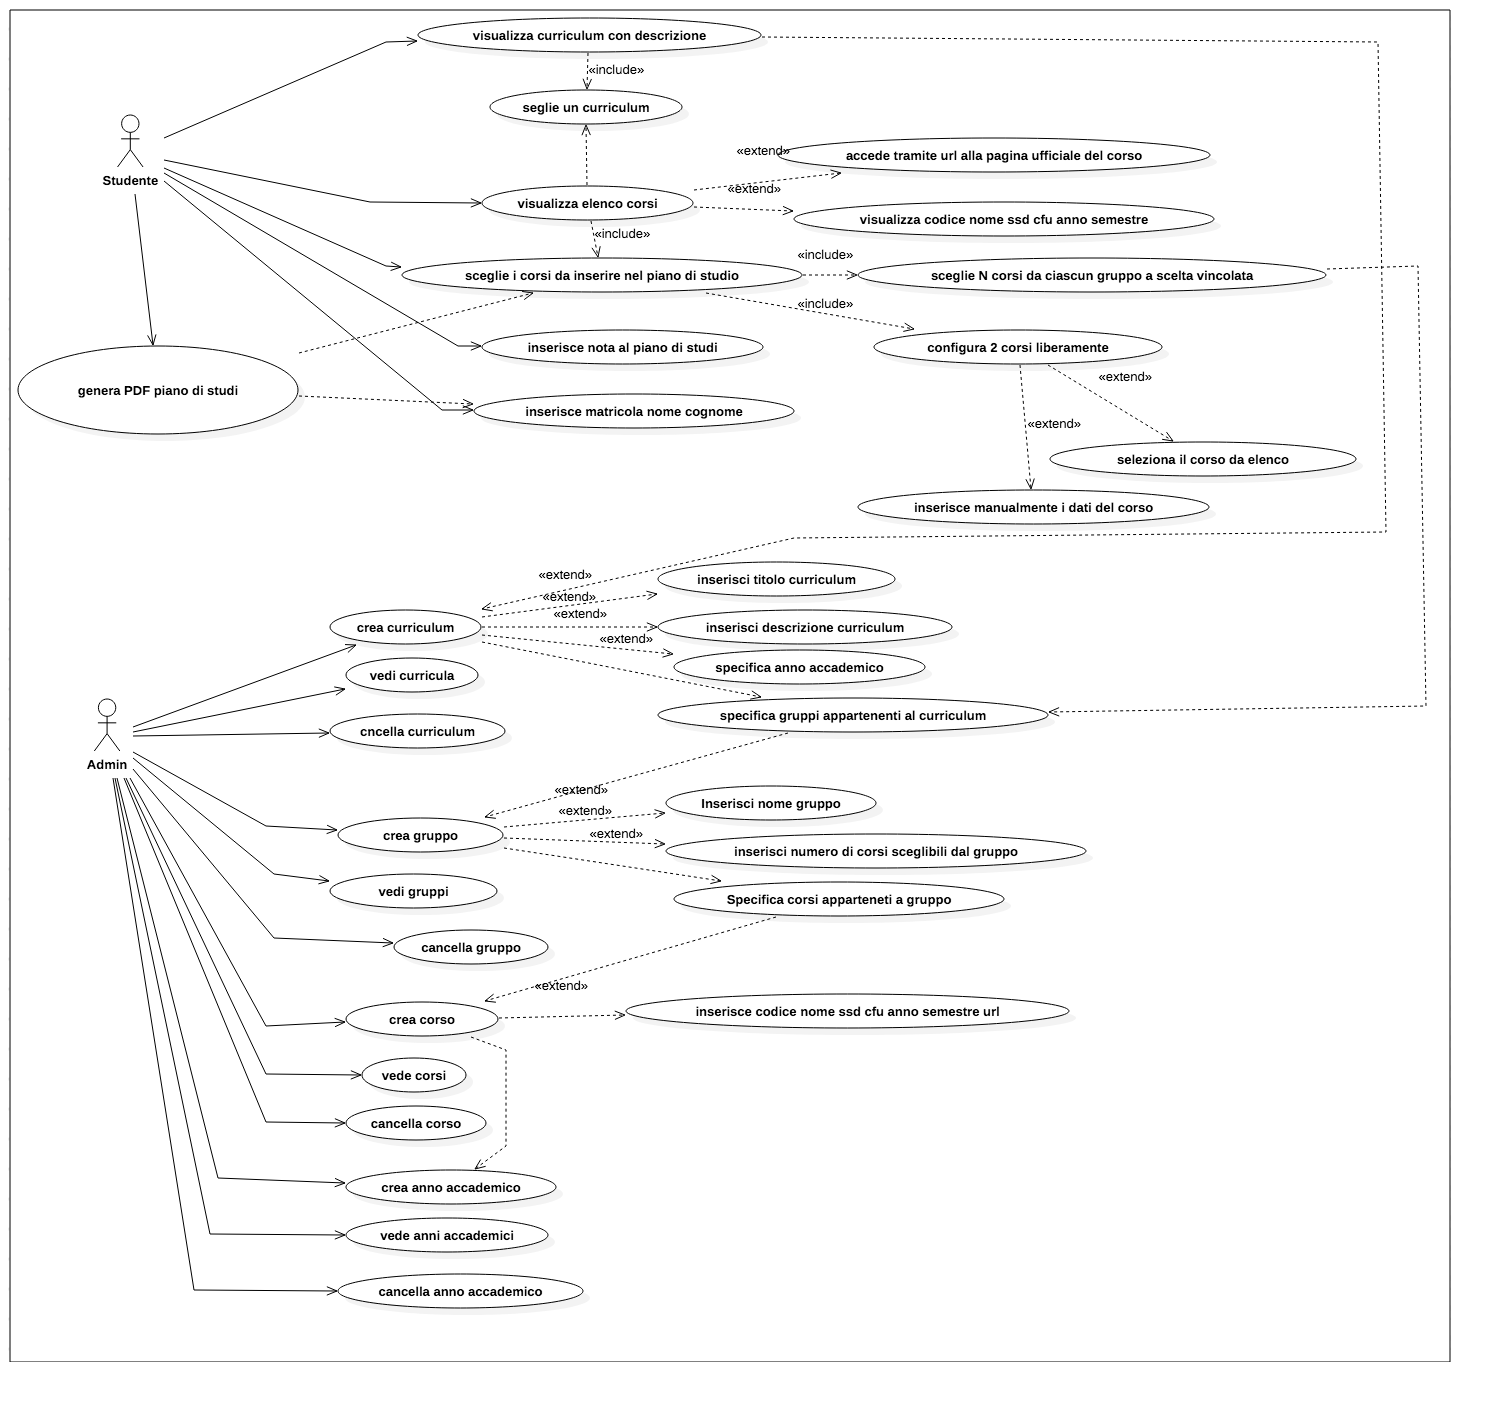
\includegraphics[width=\textwidth]{img/UseCaseDiagram.png}
     \caption{Use case diagram - simplified version}
  \label{fig:Usecasediagram}
  \end{center}
\end{figure}



\newpage
\section{Data model}
Dai requirements si sono  ricavate le seguenti entità:
\begin{itemize}
\item Student
\item Studyplan
\item Curriculum
\item Course
\item Othercourse
\item Group
\item Academicyear
\end{itemize}
\textbf{Student} modella uno studente. Lo studente è identificato da una matricola. Matricola è \emph{id} di \emph{Student}. Inoltre è caratterizzato da un nome e un cognome, \emph{firstname} e \emph{lastname}.
\\
\textbf{Studyplan} modella un piano di studi. Un piano di studi è identificato dallo studente a cui appartiene. L'\emph{id}  di \emph{Studyplan} è uguale a \emph{id} di \emph{Student}. Un piano di studi è caratterizzato da uno e un solo \emph{Curriculum}, da un certo numero di \emph{Courses} a scelta vincolata e da due corsi a scelta libera, \emph{Othercourses}. Inoltre un piano di studi può contenere una \emph{note} testuale. 
\\
\textbf{Curriculum} modella un curriculum. E' identificato da un \emph{id}, numero automaticamente dato dal sistema. Un \emph{Curriculum} è caratterizzato un titolo, una descrizione e un anno accademico, rispettivamente \emph{title, desc, ac}. Inoltre un curriculum è caratterizzato da un insieme di gruppi. vedi \emph{Group}. 
\\
\textbf{Group} è un raggruppamento di corsi scelti dall'amministratore secondo un criterio di affinità degli stessi. Un gruppo serve a definire i criteri di selezione dei corsi a scelta. vincolata. Ciascun gruppo è caratterizzato da un \emph{name} con funzione descrittiva, per esempio 'gruppo Automazione 01'.  A ciascun gruppo è associato un insieme di \emph{Courses}. In analogia a quanto avviene nei piani di studio cartacei, un \emph{Group} rappresenta una tabella di corsi a scelta vincolata all'interno del quale lo studente deve scegliere obbligatoriamente  \emph{n}  corsi tra quelli contenuti nel gruppo. \emph{Group} è identificato da un \emph{id}, numero automaticamente dato dal sistema.  
\\
\textbf{Course} Rappresenta un corso a scelta vincolata appartenente all'insieme dei corsi disponibili per la scuola a cui è rivolta l'applicazione, in questo caso la scuola di ingegneria informatica dell'università di Firenze. \emph{Course} è creato dall'amministratore del sistema ed inserito nel relativo database. Un \emph{Course} è identificato da un codice corso, un nome, un settore disciplinare, un numero di cfu, un anno accademico,  l'anno ed il semestre in cui è previsto lo svolgimento del corso ed un url alla pagina ufficiale del corso, rispettivamente \emph{id, name, ssd, cfu, ac, year, semester, url}.
\\
\textbf{Othercourse} Rappresenta un corso a scelta libera che può non appartenere ai corsi disponibili per la scuola considerata, da cui il nome \emph{Othercourse}. I corsi presenti in \emph{Othercourse} sono creati dallo studente ed inserti nel relativo database. Questi corsi hanno un numero di attributi minore rispetto a \emph{Course}. In particolare sono  composti da  un codice corso, un nome, un settore disciplinare, un numero di cfu, rispettivamente  \emph{id, name, ssd, cfu}.
\\
\textbf{Academicyear} consiste in una stringa che rappresenta l'anno accademico (i.e 2018-2019) ed è anche identificativa per l'entità.


\begin{figure}[H]
  \begin{center}
   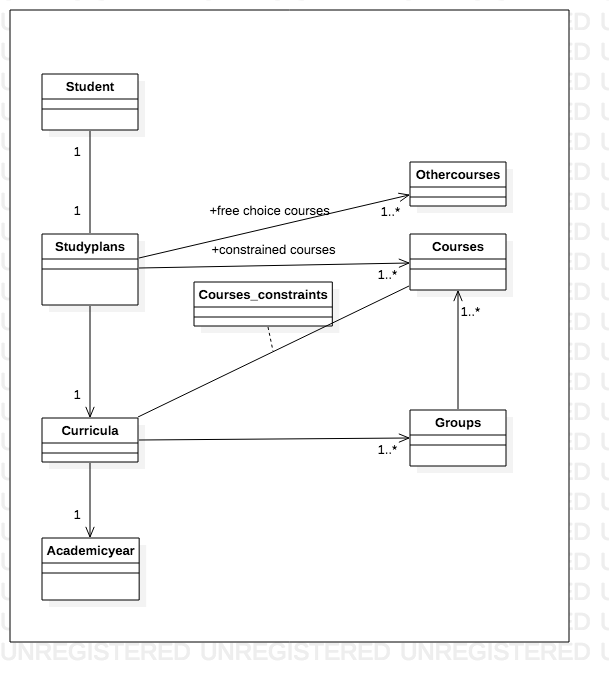
\includegraphics[width=.6\textwidth]{img/UMLconcettuale.png}
     \caption{UML concettuale}
  \label{fig:EntityRelationshipdiagram1}
  \end{center}
\end{figure}

Dai casi d'uso in \ref{fig:Usecasediagram} sono stati ricavate le relazioni mostrate in figura \ref{fig:EntityRelationshipdiagram1}
\begin{table}[!h]
  \begin{center}
    \caption{Entity relations}
    \label{tab:Entity Relationship}
    \begin{tabular}{l|l} % <-- Alignments: 1st column center, 2nd left
      \textbf{ER} & \textbf{cardinality}  \\ 
      \hline
		Student - Studyplans & one-to-one bidirectional \\
		Studyplans - Curricula & many-to-one bidirectional\footnote{La bidirezionalità da curriculum a piano di studi serve a permettere la cancellazione di un curriculum. Vedi note su cancellazione. } \\
		Studyplans - Courses  & many-to-many unidirectional \\
		Studyplan - Othercourses & many-to-many unidirectional \footnote{many-to-two} \\
		Curricula - Groups & many-to-many unidirectional \\
		Groups - Courses & many-to-many unidirectional \\
    \end{tabular}
  \end{center}
\end{table}

In particolare si evidenziano le osservazioni:
\begin{itemize}
\item \textbf{Student - Studyplan}: Ad uno studente deve corrispondere uno e un solo piano di studi. Ad un piano di studi deve corrispondere uno e un solo studente. la relazione è stata modellata in modo bidirezionale, così che da uno studente si possa ricavare il suo piano di studi e viceversa. Se cancello uno studente  cancello il suo piano di studi e se cancello un piano di studi cancello lo studente a cui appartiene.
\item \textbf{Studyplan - Curricula }: Ad un piano di studio deve corrispondere uno e uno solo curriculum. Un curriculum è in uso su zero o molti piani di studio. Sebbene dai casi d'uso non sia emersa la necessità di sapere i piani di studio associati ad un curriculum, questa relazione è stata fatta bidirezionale per consentire l'eliminazione di un curriculum; Per cancellare un curriculum e non violare i vincoli di integrità  (foreign key su \emph{Studyplan}) è infatti necessario avere una relazione tra curriculum e piani di studio. Si sottolinea che così facendo l'eliminazione di un curriculum renda nullo il campo \emph{curriculum\_id} in tutti i piani di studio che lo avevano scelto. Questa opzione è stata considerata accettabile in fase di progettazione. D'altra parte l'amministratore deve avere totale controllo sulla eliminazione dei curricula. Inoltre se l'amministratore decide di eliminare un curriculum, i piani di studio che lo avevano scelto non saranno più validi.
\item \textbf{Studyplan - Courses}:  Ad un piano di studi devono corrispondere uno o più corsi a scelta vincolata. Un corso sarà incluso in zero o molti piani di studio.  La relazione è stata fatta unidirezionale perché non esiste un caso d'uso che richiede di sapere i piani di studio associati ad un corso. Quando l'amministratore elimina un corso, quel corso è automaticamente rimosso dai piani di studio che lo  avevano scelto.
\item \textbf{Studyplan - Courses}:  Ad un piano di studi devono corrispondere due corsi  a scelta libera.
\item \textbf{Curricula - Groups}: Un curriculum è fatto di uno o più gruppi. Un gruppo può essere incluso in zero o molti curricula. La relazione è stata fatta unidirezionale perché non esiste un caso d'uso che richieda di sapere i curricula associati ad un gruppo. L'eliminazione di un gruppo provoca la rimozione di quel gruppo dai curricula.
\item \textbf{Groups - Courses }: Un gruppo è fatto da uno o più corsi. Gruppi diversi possono avere alcuni corsi in comune (a patto che questi gruppi non appartengano ad uno stesso curriculum ). Anche in questo caso non esiste un caso d'uso che richieda di sapere, dato un corso, quali gruppi appartengono a quel corso.
\end{itemize}
La figura \ref{fig: Entity Relationship diagram} illustra il diagramma ER in prospettiva di implementazione.\\
Il database è stato realizzato in \texttt{Postgres} tramite \texttt{SQLAlchemy} in \texttt{Python Flask}.




\begin{sidewaysfigure}
  \centering
   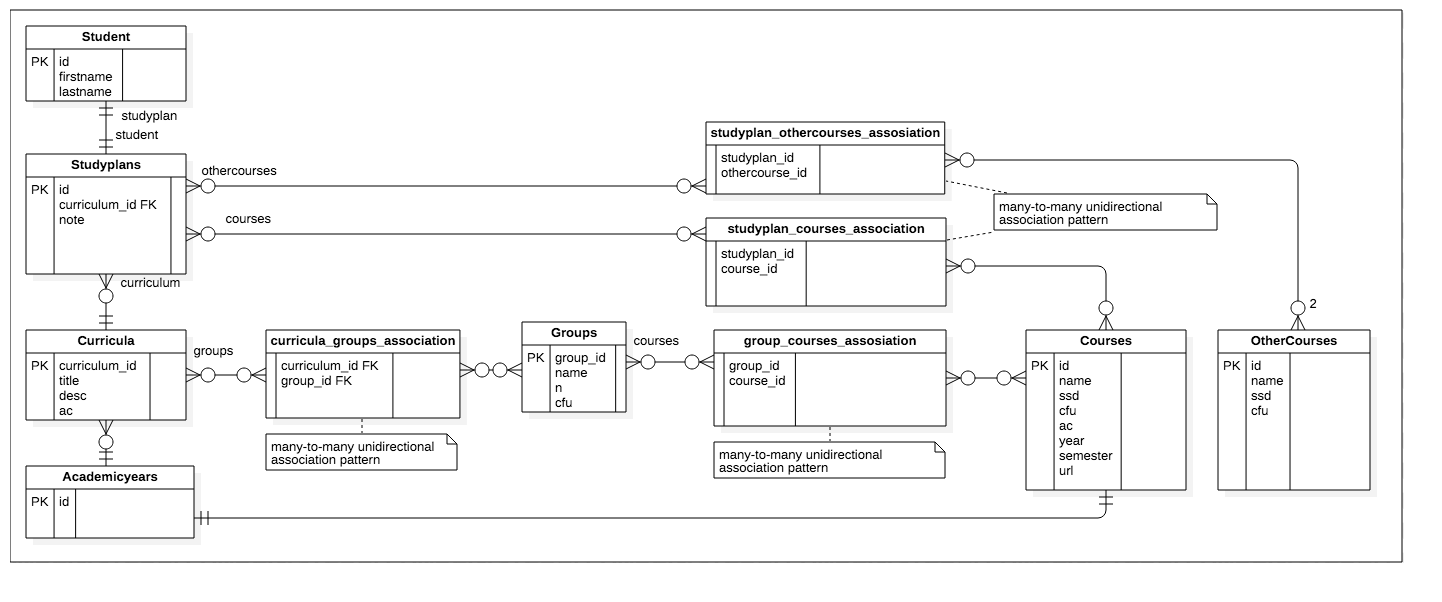
\includegraphics[height=10cm]{img/ERD.png}
     \caption{ER diagram}
  \label{fig: Entity Relationship diagram}
\end{sidewaysfigure}

\newpage

\section{Creazione e validazione delle entità}
\begin{itemize}
\item \textbf{Academicyear}
Nel caso di \emph{ Academicyear} l'id è del tipo \texttt{2018-2019}.  La validazione consiste nel:
\begin{enumerate}
\item controllare che il valore sia non nullo
\item controllare che  il carattere '-' separi gli anni.
\item controllare che l'anno indicato si trovi in un range di valori ragionevoli, nel caso tra  2018 e 2022
\item controllare che l'anno successivo al primo sia quello successivo.
\end{enumerate}
\item \textbf{Course}
Nel caso di \emph{Course} l'id è del tipo \texttt{B012345}. La validazione consiste nel
\begin{enumerate}
\item controllare che il valore sia non nullo
\item controllare che il codice abbia esattamente 7 caratteri
\item controllare che il nome del corso non sia vuoto
\item controllare che il numero dei cfu sia o 6 o 9
\item controllare che il campo ssd non sia vuoto
\end{enumerate}
\item \textbf{Group}
\begin{enumerate}
\item controllare che il nome del gruppo non sia vuoto
\item controllare che il gruppo non sia privo di corsi
\item controllare che il numero di corsi da scegliere nel gruppo non sia zero
\item controllare che il numeri di corsi presenti nel gruppo sia superiore al minimo numero di corsi che lo studente può scegliere da quel gruppo.
\end{enumerate}
Nota: L'unicità dei corsi in un gruppo è verificata all'interno di curriculum.
\item \textbf{Curriculum}
\begin{enumerate}
\item controllare che il titolo sia non nullo
\item controllare che il curriculum non sia privo di gruppi
\item controllare che non ci siano corsi uguali per id in gruppi diversi, ovvero che i corsi di un curriculum siano unici
\item controllare che corsi e cfu specificati dal gruppo siano sufficienti a totalizzare 84 cfu ( numero di crediti dei corsi a scelta vincolata)
\end{enumerate}
Nota: Il controllo sulla unicità del corso è stato inserito in considerazione del fatto che dalle tabelle riportate nei requirements non si è visto nessun corso duplicato in più gruppi all'interno di un curriculum.
\item \textbf{Student}
Nel caso di \emph{Student} l'id è del tipo \texttt{1234567}. La validazione consiste nel
\begin{enumerate}
\item controllare che il valore sia non nullo
\item controllare che il codice abbia esattamente 7 caratteri
\end{enumerate}
\item \textbf{Studyplan}
Nel caso di \emph{Studyplan} non è necessario controllare l'id in quanto vincolato all'id dello \emph{Student}.
La validazione consiste nel:
\begin{enumerate}
\item verificare che non ci siano corsi duplicati ( unicità del corso ).
\item verificare che per ogni gruppo del curriculum siano stati scelti almeno n corsi.
\end{enumerate}
\end{itemize}

\begin{figure}[H]
  \begin{center}
   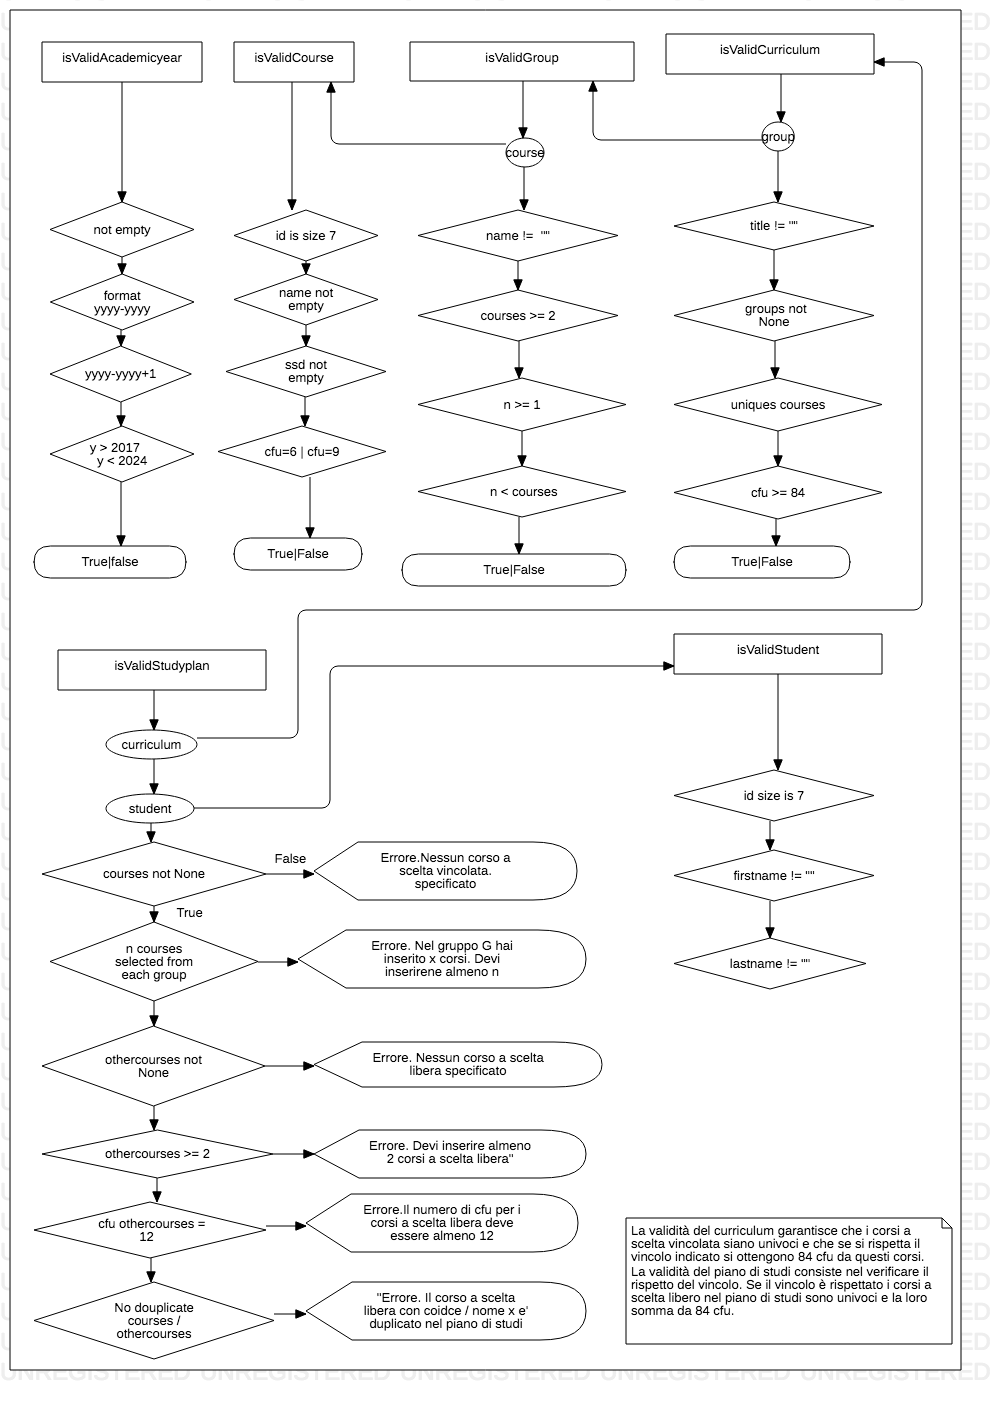
\includegraphics[width=\textwidth]{img/validazione.png}
     \caption{Validazione - Flow diagram}
  \label{fig:ValidationFlowDiagram}
  \end{center}
\end{figure}

\newpage
\subsection{Creazione e cancellazione di entità e relazioni  in SQLAlchemy }
La creazione di una entità deve rispettare l'ordine di creazione delle entità da cui dipende. Il motivo per cui non si è potuto fare altrimenti è che la validazione di una entità dipende per lo più dai dati delle altre entità. Ad esempio, la validazione del curriculum richiede che siano noti i corsi che fanno parte di quel curriculum. Per evitare la possibilità di creare entità non valide si è preferito costringere l'amministratore ad eseguire la creazione ordinata delle entità.
In particolare si evidenzia che l'ordine di creazione delle entità deve rispettare il seguente ordine:
\begin{enumerate}
\item Creazione dell'anno accademico \emph{Academicyears}
\item Creazione dei corsi \emph{Courses}
\item Creazione dei gruppi \emph{Groups}
\item Creazione dei curricula \emph{Curricula}
\item creazione di \emph{Othercourses}
\item creazione di \emph{Student}
\item creazione di \emph{Studyplans}
\end{enumerate}

Per quanto riguarda la cancellazione delle entità, il sistema è stato progettato per permettere all'amministratore la cancellazione di tutte le entità della base di dati. L'inconsistenza dei vincoli espressi nelle relazioni è verificata a livello applicativo.\\ Di seguito sono analizzate le relazioni.
In particolare si evidenzia che: \\
\begin{itemize}
\item \textbf{curricula-groups}  Many-to-Many unidirectional association pattern con padre Curricula e figlio Groups.
La cancellazione di un gruppo da parte dell'amministratore provoca la rimozione di quel gruppo dai curricula che lo contenevano ma non la cancellazione del curricula. Tuttavia può darsi che la cancellazione di un gruppo da un curriculum invalidi il curriculum a causa del non raggiungimento degli 84 cfu necessari.
\begin{python}
class Curricula(Base):
    __tablename__ = 'curricula'
	...
    groups = db.relationship('Groups', secondary='curricula_groups_association')
    
curricula_groups_association = db.Table('curricula_groups_association', Base.metadata,
    db.Column('curriculum_id', db.Integer, db.ForeignKey('curricula.id')),
    db.Column('group_id',  db.Integer, db.ForeignKey('groups.id',  ondelete='cascade')))
\end{python}

\item \textbf{groups-courses} Many-to-Many unidirectional association pattern con padre Groups e figlio Courses.
La cancellazione di un corso provoca la rimozione di quel corso dai gruppi che lo contenevano. Occorre verificare che il gruppo sia ancora valido. In particolare che il numero di corsi presenti nel gruppo sia superiore al numero di corsi obbligatori da scegliere.
\begin{python}
class Groups(Base):
    __tablename__ = 'groups'
	...
    courses = db.relationship('Courses', secondary='groups_courses_association')

groups_courses_association = db.Table('groups_courses_association', Base.metadata,
    db.Column('group_id', db.Integer, db.ForeignKey('groups.id')),
    db.Column('course_id', db.String(7), db.ForeignKey('courses.id',  ondelete='cascade')))
\end{python}

\item \textbf{studyplan-courses}  Many-to-Many unidirectional association pattern con padre  Studyplan e figlio Courses.
La cancellazione di un corso da un piano di studi invalida il piano di studi ma non lo cancella. Si assume che lo scopo dell'applicazione è quello di favorire lo studente nella creazione del PDF relativo al piano di studi. Lo studente che accede all'applicazione in un dato momento configura il proprio piano di studi con i corsi  presenti nel database in quel momento. Se, a distanza di un anno dal primo piano di studi creato, lo studente  intende rinnovare il piano di studi per l'anno successivo dovrà compilarlo ex-novo con i corsi disponibili nel sistema. 
\begin{python}
class Studyplans(Base):
    __tablename__ = 'studyplans'
	..
    courses = db.relationship('Courses', secondary='studyplan_courses_association')
    
studyplan_courses_association = db.Table('studyplan_courses_association', Base.metadata,
    db.Column('studyplan_id', db.String(7), db.ForeignKey('studyplans.id')),
    db.Column('course_id', db.String(7), db.ForeignKey('courses.id',  ondelete='cascade')))
\end{python}


\item \textbf{studyplan-othercourses} Many-to-Many unidirectional association pattern con padre  Studyplan e figlio Othercourses
Nel sistema non è stato implementato nessun meccanismo di cancellazione dei corsi dalla tabella othercourses. 
\begin{python}
class Studyplans(Base):
    __tablename__ = 'studyplans'
	..
    othercourses = db.relationship('OtherCourses', secondary='studyplan_othercourses_association')

studyplan_othercourses_association = db.Table('studyplan_othercourses_association', Base.metadata,
    db.Column('studyplan_id', db.String(7), db.ForeignKey('studyplans.id')),
    db.Column('othercourse_id', db.String(7), db.ForeignKey('othercourses.id',  ondelete='cascade')))
\end{python}

\item \textbf{studyplan-curriculum} Many-to-one bidiectional pattern.
In questo caso la bidirezionalità, in particolare da curriculum verso studyplan, è stata aggiunta per permettere all'amministratore di cancellare i piani di studio che rimangono senza curriculum a seguito della cancellazione dello stesso. 
\textcolor{red}{La scelta di cancellare i piani di studi riferiti a curriculum non più esistenti serve a mantenere pulito il database, dando modo all'amministratore di rimuovere i piani di studi obsoleti.}
\begin{python}
class Studyplans(Base):
    __tablename__ = 'studyplans'
	..
    curriculum = db.relationship('Curricula', backref=db.backref('studyplans', uselist=False,  cascade='all,delete'))
\end{python}

\item \textbf{Studyplan-Student} One-to-One bidirectional pattern con padre Student e figlio Studyplan
Studente e piano di studi sono fortemente accoppiati. Se cancello il piano di studio, cancello anche lo studente che lo possiede.
L'inserimento di ondelete='Cascade' all'interno della ForeignKey è stato aggiunto per conferire robustezza al codice; non esiste un meccanismo che permette la cancellazione  diretta dello studente. Solo in seguito a cancellazione di un curriculum, studenti e piani di studio possono essere cancellati dall'amministratore.
\begin{python}
class Studyplans(Base):
    __tablename__ = 'studyplans'
    id = db.Column(db.String(7), db.ForeignKey('students.id', ondelete='CASCADE'), primary_key=True)
    student = db.relationship('Students', backref=db.backref('studyplans', uselist=False), cascade='delete')
\end{python}
\end{itemize}
\newpage


\section{Page navigation diagram}
\begin{table}[!h]
  \begin{center}
    \caption{Page navigation}
    \label{tab:Page navigation}
    \begin{tabular}{l|l} % <-- Alignments: 1st column center, 2nd left
      \textbf{directory} & \textbf{descrizione}  \\ 
      \hline
		/ & vedi elenco dei curricula e scegli curriculum\\
		/curriculum/1 & vedi corsi disponibili per curriculum, seleziona corsi e  inserisci dati per piano di studi\\
		/studyplan/1234567  & vedi piano di studi e stampa pdf \\
		/admin/index & vedi pannello di controllo \\
		/admin/passwd  & cambia credenziali di accesso dell'amministratore\\
		/admin/course/index & Vedi lista dei corsi disponibili e accedi alle opzioni CRUD per corsi \\
		/admin/course/create & Inserisci dati per creazione di un nuovo corso \\
		/admin/course/read/1 & Leggi dettagli corso \\
		/admin/course/delete/1 & Cancella corso \\
		/admin/group/index & Vedi lista dei gruppi disponibili e accedi alle opzioni CRUD per gruppi \\
		/admin/group/create &  Inserisci dati per creazione di un gruppo \\
		/admin/group/read/1 & Leggi dettagli gruppo \\
		/admin/group/delete/1 & Cancella gruppo \\
		/admin/curriculum/index & Vedi lista dei curriculum disponibili e accedi alle opzioni CRUD per curriculum \\
		/admin/curriculum/create &  Inserisci dati per creazione di un nuovo \\
		/admin/curriculum/read/1 & Leggi dettagli curriculum \\
		/admin/curriculum/delete/1 & Cancella curriculum \\
		/admin/studyplan/index & Vedi tutti i piani di studio \\
		/admin/studyplan/read/5972786 & vedi dettagli del piano di studi \\
		
    \end{tabular}
  \end{center}
\end{table}

\newpage

\section{Autenticazione admin}
L'autenticazione è stata implementata tramite Flask simple login\cite{rif5}.
Ad ogni operazione di creazione o cancellazione di entità è stato aggiunto il decoratore
\begin{python}
@login_required
\end{python}
Tramite questo decoratore quando si prova ad accedere all'url protetto da login si viene reindirizzati ad una pagina di login in cui inserire username e password. Successivamente l'applicazione manterrà valida l'autenticazione per la durata della sessione.\\
La prima volta che viene fatta partire l'applicazione username e password sono inizializzati ad 'admin - admin'.
\begin{python}
def init_user_password():
    if  Admin.query.get(0) is None:
        username = 'admin'
        password = generate_password_hash('admin', method='pbkdf2:sha256')
        admin = Admin(idd=0, username=username, password=password) 
\end{python}
Successivamente tramite interfaccia grafica alla pagina /admin/passwd sarà possibile modificare username e password con valori a propria scelta.
Si noti che:
\begin{itemize}
\item La password non è memorizzata in chiaro. Viene memorizzato il digest dell'hash.
\item La tabella Admin ammette un solo utente ( con id=0)
\end{itemize}

\newpage
\section{CSV Parser}
A partire dal file csv fornito si è implementato uno script python che effettua il parse dei dati del csv e crea automaticamente i corsi.

\begin{python}[caption=Data parser]
csvfile = open("csv/corsi.csv", "r") 
csvfile.readline() 
for line in csvfile:
	row = line.split(";")
\end{python}
Lo script esclude dal parser i due casi di 'non corso': Uno riguarda la prova finale e l'altro il laboratorio\/tirocinio.
Oltre che per una questione logica, i due devono essere evitati perché non avendo il campo 'semestre' mandano in errore il parser.
Inoltre le 'string' analizzate post-parser includono l'aggiunta di uno spazio vuoto a fine della parola. Leliminazione dello spazio è eseguito con:
\begin{python}[caption=String manupulation]
		id = row[3]
		id = id[:-1]
		ssd = row[5]
		ssd = ssd[:-1]
		name = row[4]
		name = name[:-1]
\end{python}
L'anno accademico è inserito da admin da interfaccia grafica. L'url che non è disponibile è momentaneamente settato con link a pagina interna.
\begin{python}
                url = "#"
                ac = request.form['academicyear']
\end{python}
\section{Generazione del pdf relativo al piano di studi}
La generazione del pdf lato server richiede l'installazione dell'applicazione
\begin{shell}
sudo apt-get install wkhtmltopdf
\end{shell}
La creazione del pdf e l'invio dello stesso al client è gestita da:
\begin{python}
	studyplanDoc = render_template('studyplan.html', studyplan=studyplan, student=student)
    pdf = pdfkit.from_string(studyplanDoc, False)
    response = make_response(pdf)
    response.headers['Content-Type'] = 'application/pdf'
    response.headers['Content-Disposition'] = 'inline; filename=pianodistudi.pdf'
\end{python}

\newpage
\section{Guida all'installazione dell'applicazione}
Prima di procedere al setup assicurarsi di avere Python e pip installati. ( io ho python \textit{2.7.10} e pip \textit{18.0} ) 
\begin{shell}[caption=Setup Flask]
mkdir curriculaWebApp && cd curriculaWebApp
pip install virtualenv
virtualenv env
source env/bin/activate
git init
git clone https://github.com/FrancescoErmini/CurriculaWebApp4.git
export FLASK_APP=app.py
pip install Flask
pip install -r requirements.txt
\end{shell}
Poi dopo aver scaricato Postgres sul  proprio sistema operativo, accedere alla console \emph{psql}, quindi creare un database, creare un utente e associare utente al database.
\begin{shell}[caption=Create database]
CREATE USER pala WITH PASSWORD 'password';
CREATE DATABASE pianodistudio2;
GRANT ALL PRIVILEGES ON DATABASE pianodistudio2 TO pala;
\end{shell}
in alternativa, scaricare \textbf{pgAdmin 4} e fare tutto graficamente.\\
Prima di procedere oltre verificare che nel file \emph{app.py} i dati inseriti sopra siano corretti:
\begin{python}[firstnumber=16, caption=Flask db configuration]
POSTGRES = {
    'user': 'pala',
    'pw': 'password'
    'db': 'pianodistudio2',
    'host': 'localhost',
    'port': '5432',
}
app.config['DEBUG'] = True
app.config['SQLALCHEMY_DATABASE_URI'] = 'postgresql://%(user)s:\
%(pw)s@%(host)s:%(port)s/%(db)s' % POSTGRES
\end{python}
A questo punto si procede alla migrazione del database seguendo lo schema di migrazione \cite{ref1}. 
\begin{shell}[caption=Initialize database]
python manage.py db init
python manage.py db migrate
python manage.py db upgrade
python manage.py runserver
\end{shell}
In aggiunta occorre installare su Debian/Ubuntu una applicazione che si occupa della creazione del pdf lato server:
\begin{shell}
sudo apt-get install wkhtmltopdf
\end{shell}
\subsection{Deploy dell'applicazione su Server Ubuntu}
Per le istruzione sul deploy si rimanda alla guida:
\url{https://medium.com/ymedialabs-innovation/deploy-flask-app-with-nginx-using-gunicorn-and-supervisor-d7a93aa07c18}



\newpage
\begin{thebibliography}{Bibliografia}
\bibitem{rif1}  Flask migration \url{https://medium.com/@dushan14/create-a-web-application-with-python-flask-postgresql-and-deploy-on-heroku-243d548335cc}
\bibitem{rif2}  Many-to-Many in SQLAlchemy  \url{http://docs.sqlalchemy.org/en/latest/orm/basic_relationships.html#many-to-many}

\bibitem{rif3}  Flask Tutorial \url{https://danidee10.github.io/2016/09/19/flask-by-example-2.html}
\bibitem{rif4}  Base class schema in SQLAlchemy \url{https://medium.com/@lsussan/base-classes-one-to-many-relationships-in-flask-sqlalchemy-fba0d47374ad}
\bibitem{rif5} Flask simple login \url{https://github.com/rochacbruno/flask_simplelogin}
\end{thebibliography}

\end{document}
